\documentclass[tikz,border=1pt]{standalone}
\usepackage{tikz}

\tikzset{every node/.style={shape=circle,draw = black}}
\tikzset{every edge/.style={draw = red, very thick}}
\begin{document}
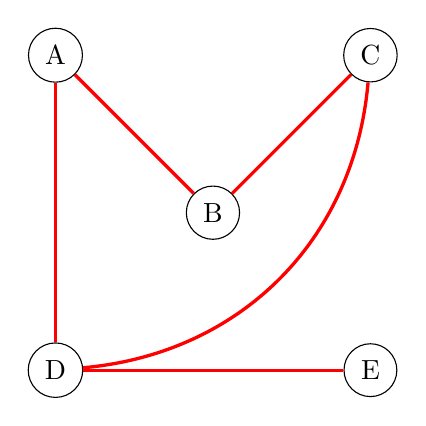
\begin{tikzpicture}[node distance = 2cm]
  \node (A) {A};
  \node (B) [right of= A,below of = A] {B};
  \node (C) [right of = B,above of = B] {C};
  \node (D) [node distance = 4cm, below of = A] {D};
  \node (E) [node distance = 4cm, right of = D] {E};

  \path (A) edge (B);
  \path (A) edge (D);

  \path (B) edge (C);

  \path (C) edge[bend left = 40] (D);

  \path (D) edge (E);
\end{tikzpicture}

\end{document}
